\subsection{Evaluation Methodology:}
Evaluating the application is done by two methods both based upon methods found in the literature review.
The first is a visual test at time steps during the running of the program.
This will showcase the formation and deformation of clouds and the generation of rain.
Figure \ref{fig:Simple Realistic Animation of Clouds} shows \citet{DobashiEtAl00}) results in the manner describe here.
In the appendix Figure \ref{fig:A_Method_for_Modeling_Clouds_based_on_Atmospheric_Fluid_Dynamics} to Figure \ref{fig:Simulation_of_Cloud_Dynamics_on_Graphics_Hardware} show the results from other models.
This method has been chosen because it shows of the purpose of the project which is to have visually realistic clouds simulated at real time with the creation of rain.

\begin{figure}[h!]
  \centering
  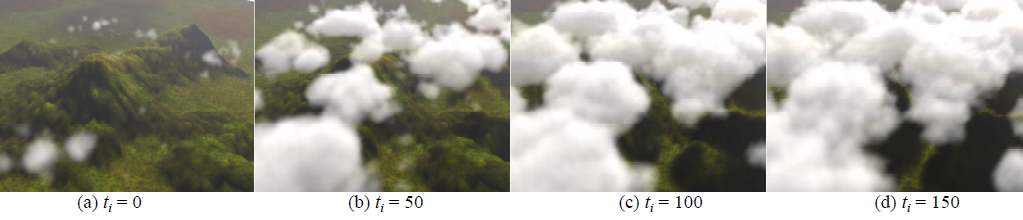
\includegraphics[width=140mm]{images/Simple_Realistic_Animation_of_Clouds.PNG}
  \caption{\citet{DobashiEtAl00}}
  \label{fig:Simple Realistic Animation of Clouds}
\end{figure}

The other method for testing the application is to test how much resources are being used by the application.
\citet*{MHarris01}, and \citet{Elek12} both used this method when evaluating their models.
This form of evaluation tests how efficient the application is when running in real time as well as concerns like the size of grid that can be used.
This can be accomplished using \citet*{nvidiasight2013} for debugging CUDA and profiling the application.